\documentclass[Main/main.tex]{subfiles}

\begin{document}
%\vspace{-20pt}
\chapter{Introduction}

%Define and delimit the problem
%Point out the motivation of the study
%General theoretical background
%Science perspective


The work in this thesis consists of two parts, exploration of a new liquid injection system for the synthesis of oxides and application of this method to synthesize cathode materials directly on a current collector. These novel cathodes will not need a traditional binder in order for the cathode material to stick to the conducting surface. If this method proves to be tunable and replicable, cathodes produced by liquid injection may be able to compete with present cathodes.

Today, we surround ourselves with electricity - from electrical watches and smartphones to electrical cars and power grids. The aim for a more environmental-friendly future, together with the increasing complexity and finesse of electrical devices calls for a constant development of our technology for storing electrical energy and converting it into a usable form when required - the battery.

Batteries are commonly divided into two categories; primary and secondary batteries. Primary batteries cannot be electrically recharged and are therefore single use, whereas secondary batteries are rechargeable. The latter can offer savings in costs and resources since the batteries can be re-used instead of just disposed of when empty. A battery consists of three major parts; the anode, the electrolyte and the cathode. The cathode plays an important role when it comes to improving various aspects of batteries, such as cost, safety, power and energy densities \cite{gandrud}. Nowadays, the cathode is typically the most costly element, comprising about 30 \% of the total price of the battery \cite{costcath}. Moreover, as shown in figure \ref{fig:1_discharge_specific}, present cathode materials exhibit around half the specific capacity as the carbon anodes used today \cite{1_rev_liion}. Consequently, in order to develop batteries fit for the next generation electric vehicles and energy storage systems, research into cathodes is paramount.

\begin{figure}[ht]
    \resizebox{\textwidth}{!}{
	\begin{subfigure}[t]{0.5\textwidth}
		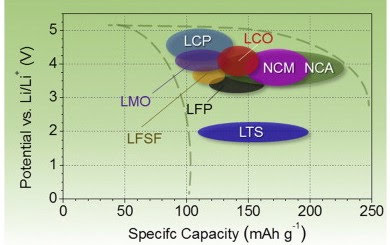
\includegraphics[scale=0.5825]{uploads/1_discharge_specific_cathode} %61
		\caption{Intercalation-type cathodes}
		\label{fig:1_dis_a}
	\end{subfigure}
	~ 
	\begin{subfigure}[t]{0.5\textwidth}		
		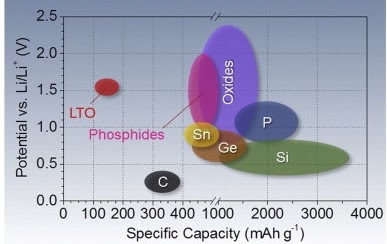
\includegraphics[scale=0.585]{uploads/1_discharge_specific_anodes} %6125
		\caption{Converson-type anodes}
		\label{fig:1_dis_b}
	\end{subfigure} }
    \caption{Approximate range of average discharge potentials and specific capacity of some of the most common electrodes in todays researched and commercial batteries \cite{1_rev_liion}.}
    \label{fig:1_discharge_specific}
\end{figure}

\newpage
\section{History}

The first electrical battery is credited to the Italian physicist Alessandro Volta who, in 1800, invented the Voltaic pile consisting of alternating disks of zinc and copper separated by brine-soaked paper \cite{1_volta}.\  Since then, a lot of different chemistries and structures have been tested. Among these we find the first rechargeable battery invented in 1859, the lead-acid battery, which to present day is being used to start internal combustion engine cars. In 1957, the typically non-rechargeable alkaline battery used in regular household devices saw the light of day. \cite{1_yazami}

The next big breakthrough, however, came from Sony Corporation in 1991 with the pairing of a \ce{LiCoO2} (LCO) cathode and a graphite anode to manufacture and commercialize the first mass-produced rechargeable lithium battery \cite{1_hist}. Li-ion batteries had been researched since 1970, starting with fundamental research into intercalation of Li into layered transition-metal sulfides and selenides \cite{Goodenough2013}. Unfortunately, during recharging of these batteries, dendritic growth of Li occurred, causing the battery to short circuit by connecting the electrodes through the electrolyte solution.
In 1980, John B. Goodenough and his research group found LCO to be a stable cathode material capable of donating Li-ions. Later, in 1983, Rachid Yazami was exploring Li intercalation onto graphite and found reversible Li insertion into carbon to avoid the rather pressing problem of dendrite formation \cite{1_LIB_birth} \cite{1_yazami}. Akira Yoshino made use of these discoveries and invented the Li-ion battery as we know it today in 1985. This battery system comprised of a "non-aqueous secondary battery using transition-metal oxides containing lithium ion such as \ce{LiCoO2} as a positive electrode and carbonaceous materials as a negative electrode" \cite{1_LIB_birth}.



\section{The Li-ion battery}

The Li-ion battery (LIB) can be credited for the wireless revolution of portable computers, cell phones and tablets that has reformed global communication and is starting to reshape travel as well. As shown by companies such as Tesla, Kia and Nissan, the internal combustion engine can be replaced by a combination of a portable rechargeable battery and an electrochemical capacitor.
There are, however, some imminent questions regarding cost, safety and driving range.  

Li-ion batteries possess certain fundamental advantages compared to other chemistries. Li, being the third element in the periodic table, is the third lightest element and has one of the smallest ionic radii of any single charged ion. In addition, the reduction potential of Li is the lowest of any element, giving rise to the highest possible cell potential for Li based batteries. These factors allow Li-ion batteries to have an unmatchable combination of high capacity and power density \cite{1_rev_liion}. However, there are some concerns. At present, Li-ion batteries are costly, and a shortage of Li and some of the currently used transition metals, such as Mn, Co and Ni, may one day become an issue \cite{VIKSTROM}. Nevertheless, a significant shortage of Li is unlikely in the near future \cite{Gruber, Speirs}, leaving the transition metals used in cathodes as the biggest concern at present.



\subsection{Cathodes}

A huge variety of cathodes have been researched, including, but not limited to, intercalation cathode materials, transition metal oxides, polyanion compounds and conversion cathode materials. LCO, introduced by Goodenough and commercialized by SONY, is the first and most commercially successful type of layered transition metal oxide cathodes \cite{1_rev_liion}.

An intercalation cathode contains a solid host network that is able to store guest ions, which can be inserted into and removed from the host network reversibly. In a LIB, \ce{Li+} acts as the guest ion while the host network can be metal chalcogenides, polyanion compounds or transition metal oxides. It is common to divide intercalation compounds into crystal structures, such as layered, spinel and olivine \cite{1_rev_liion}. While the layered structure was the earliest form of intercalation compounds for cathodes in LIB, this thesis aims for various manganese oxides with the spinel structure.

An ideal cathode possesses high energy and power densities, is small and inexpensive. Cobalt, used in LCO, is expensive, environmentally hazardous and ethically troublesome. Amnesty warned about excessive use of child labour in cobalt mining in 2017 \cite{1_amnesty}. In comparison, manganese is a very cheap, naturally abundant and environmentally benign element, making Mn an excellent candidate for cheaper cathode materials.

The batteries assembled and tested for this thesis have consisted of various cathodes manufactured by liquid injection, aiming for \ce{MnO2}, \ce{LiMn2O4} and \ce{LiNi_{0.5}Mn_{1.5}O4}. An anode of lithium metal and a liquid electrolyte has been used.


\paragraph{\ce{MnO2}}~\\[0.8em]
Manganese oxides are considered to be one of the most important groups of materials in energy storage science, much credited to their low cost, a high potential for nanostructuring and great diversity in the oxidation states of Mn \cite{1_Mnox_study}. Manganese dioxide (\ce{MnO2}) has been reported as a highly promising metal oxide for new cathode materials with a theoretical capacity of 308 \si{mAh/g}. Especially nanostructured and amorphous \ce{MnO2} has received attention lately \cite{1_free_MnO2, 1_amorph_MnO2}.



\paragraph{\ce{LiMn2O4} (LMO)}~\\[0.8em]
Spinel \ce{LiMn2O4} has low toxicity, good safety performance and low cost and is thus considered to be an ideal cathode material for LIBs \cite{LNMO}. The \ce{[B2]O4} array provides a strongly bonded framework where \ce{Li+} occupy all the tetrahedral A sites. This structure improves ion flow of the electrode, resulting in lower internal resistance and improved current handling. Unfortunately, it is difficult to extract all the lithium from LMO at practical voltages, thus limiting the capacity to around 120 \si{mAh/g}. Lithium extraction from LMO occurs at approximately 4 V.

\paragraph{\ce{LiNi_{0.5}Mn_{1.5}O4} (LNMO)}~\\[0.8em]
By doping the spinel LMO with a certain amount of transition metal elements, for instance Ni, the Fermi energies of the material can be adjusted and their electrode potentials increased as desired \cite{LNMO}.

Among doped spinel cathode materials, \ce{LiNi_{0.5}Mn_{1.5}O4} (LNMO) has proved promising in terms of performance and discharge capacity \cite{LNMO}. Due to the chemical reactions taking place during cycling, LNMO shows a large charge-discharge platform at 4.7 \si{V} assigned to the redox process of \ce{Ni^{2+}/Ni^{4+}} and a small platform around 4 \si{V} attributed to the \ce{Mn^{3+}/Mn^{4+}} process. 


\section[Prior work]{Prior work - Synthesis of cathode materials}
Cathode materials can be synthesised in many ways depending on the desired active material. A very common method is to make a slurry composed of active materials, such as \ce{LiCoO2}, conductive additives and polymeric binders. The conductive additive is used to enhance the electrode conductivity. This is achieved by filling free spaces made by the grains of active material forming a continuous network until the electrical conductivity approaches that of the conducting agent \cite{1_additive}. The slurry is then spread on a current collector by tape casting and can be additionally processed in order to enhance inter-particle contact and ensure good adhesion to the current collector, for instance by roll pressing. 

Recently, in order to meet a demand for high-capacity electrode materials suitable for use in electric vehicles or energy storage systems, there has been research into alternative approaches for creating 'designer particles' and applying various nanostructures and composites \cite{elmat_sprayp}. One promising technique to achieve this is spray pyrolysis.

\subsection*{Spray pyrolysis}
Spray pyrolysis is one of many techniques developed for the preparation of particles and films. Compared to other common processes such as chemical vapour deposition (CVD) or Sol-Gel, spray pyrolysis require simple and inexpensive equipment and is advantageous in terms of high reproducibility, easy addition of doping materials and chemical homogeneity in the final product \cite{1_Pyrolysis_book}. A schematic diagram of a spray pyrolysis process is displayed in figure \ref{fig:spray}.

During the process, a precursor solution of aqueous or non-aqueous solvents is atomised in a droplet generating apparatus, carried by a gas into a heated reactor where it evaporates, leading to the formation of solid particles through drying, decomposition and crystallization \cite{elmat_sprayp,Spray_pyro}. 
When the spray collides on a surface, the atoms spread out and interacts with other adsorbed atoms. Some of the atoms may initiate the formation of an island which can grow in size and coalesce \cite{1_Pyrolysis_book}. 

Spray pyrolysis is to a great extent similar to the liquid injection system used in this thesis, with the distinction of the liquid injection system operating under vacuum. The introduction of vacuum causes the solvent to evaporate and the nitrates to decompose at lower temperatures. In addition to lowering the required temperature, this can lead to less sintering and decrease the particle size \cite{elmat_sprayp}. 

The adhesion of the synthesised particles to surfaces may be a direct consequence of the vacuum, and presents a distinction from conventional spray pyrolysis at the temperatures used in this thesis .

Some authors have proposed good adhesion to be a consequence of the solvent evaporating close to the substrate and the precursor being volatilised and adsorbed onto the surface, followed by decomposition. This would correspond to a heterogenous CVD reaction \cite{adhesion}.


\begin{figure}[ht]
    \centering
    \includegraphics{uploads/schemspray.jpg}
    \caption{Schematic diagram of the spray pyrolysis process \cite{elmat_sprayp}.}
    \label{fig:spray}
\end{figure}
\section{Aim of study}

The research group has developed an injection system for the synthesis of powder. This system has proved well suited to make oxides from complex precursors. Curiously, the powder seems to adhere to the surface during synthesis. This is an effect that could prove useful to exploit for the purpose of making cathode materials for LIBs which naturally adhere to the current collector, thus not requiring any post-synthesis treatment or the addition of a polymeric binder in the synthesis. 

The research performed in this thesis aims at exploring the novel method of liquid injection in vacuum and see the effects of varying different parameters. Furthermore, to utilize the system to synthesise oxides directly on conducting steel plates and assemble batteries with the as-deposited oxides as cathode materials. Electrochemical, structural and morphological studies will be performed to assess the products.



\end{document}